\documentclass{article}
\usepackage{cmap}
\usepackage[utf8]{inputenc}
\usepackage[english,ukrainian]{babel}
\usepackage{graphicx}
\usepackage{geometry}
\usepackage{listings}
\usepackage{float}
\usepackage{amsmath}
\geometry{
	a4paper,
	left=20mm,
	right=20mm,
	top=15mm,
	bottom=15mm,
}
\lstset{
	language=c,
	tabsize=4,
	keepspaces,
	showstringspaces=false,
}
\graphicspath{ {./pictures} }
\setlength{\parindent}{4em}

\newcommand\subject{Організація комп’ютерних мереж}
\newcommand\lecturer{асистент кафедри ПЗ \\ Задорожний І.М.}
\newcommand\teacher{асистент кафедри ПЗ \\ Задорожний І.М.}
\newcommand\mygroup{ПЗ-22}
\newcommand\lab{4}
\newcommand\theme{Дослідження роботи DNS сервера та протоколу DHCP}
\newcommand\purpose{Вивчити принципи роботи DNS, на практиці ознайомитися з принципами роботи DNS-клієнта на прикладі утиліти nslookup, детально дослідити формат DNS-запиту (і відповіді) за допомогою Wireshark і nslookup, а також ознайомитися з DHCP повідомленнями}

\begin{document}
\begin{normalsize}
	\begin{titlepage}
		\thispagestyle{empty}
		\begin{center}
			\textbf{МІНІСТЕРСТВО ОСВІТИ І НАУКИ УКРАЇНИ\\
				НАЦІОНАЛЬНИЙ УНІВЕРСИТЕТ "ЛЬВІВСЬКА ПОЛІТЕХНІКА"}
		\end{center}
		\begin{flushright}
			\textbf{ІКНІ}\\
			Кафедра \textbf{ПЗ}
		\end{flushright}
		\vspace{200pt}
		\begin{center}
			\textbf{ЗВІТ}\\
			\vspace{10pt}
			до лабораторної роботи № \lab\\
			\textbf{на тему}: “\textit{\theme}”\\
			\textbf{з дисципліни}: “\subject”
		\end{center}
		\vspace{112pt}
		\begin{flushright}
			
			\textbf{Лектор}:\\
			\lecturer\\
			\vspace{28pt}
			\textbf{Виконав}:\\
			
			студент групи \mygroup\\
			Коваленко Д.М.\\
			\vspace{28pt}
			\textbf{Прийняв}:\\
			
			\teacher\\
			
			\vspace{28pt}
			«\rule{1cm}{0.15mm}» \rule{1.5cm}{0.15mm} 2023 р.\\
			$\sum$ = \rule{1cm}{0.15mm}……………\\
			
		\end{flushright}
		\vspace{\fill}
		\begin{center}
			\textbf{Львів — 2023}
		\end{center}
	\end{titlepage}
		
	\begin{description}
		\item[Тема.] \theme.
		\item[Мета.] \purpose.
	\end{description}

\section*{Теоретичні відомості}
Назвіть приклади родових доменів вищого рівня. - Родові домени вищого рівня - це рівень доменної ієрархії в системі DNS, що відповідають за організацію всіх доменів на Інтернеті. До них відносяться такі приклади:
\begin{list}{}{}
\item .com - комерційні організації;
\item .org - некомерційні організації;
\item .net - мережі та провайдери Інтернету;
\item .edu - освітні заклади;
\item .gov - урядові організації;
\item .mil - військові організації;
\end{list}

Охарактеризуйте передумови виникнення DNS. - Потрібно було спростити масштабування, адже раніше існував файл hosts.txt, в якому містилася вся інформація про відповідність всіх символьних імен вузлів і їхніх IP-адрес. Цей файл зберігався на одному вузлі мережі ARPAnet і в нього при потребі вносилися зміни.

\section*{Хід виконання}

\begin{figure}[H]
	\centering
	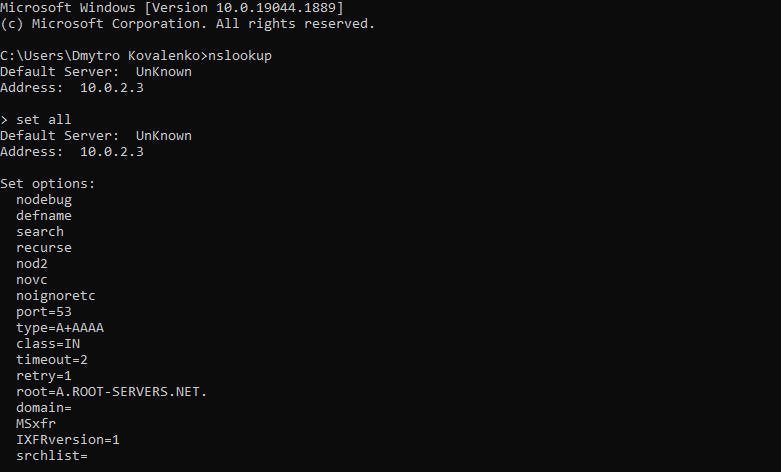
\includegraphics[width=\textwidth]{0}
	\caption{Виконання команди set all в інтерактивному режимі команди nslookup}
\end{figure}
 
 \begin{figure}[H]
 	\centering
 	\begin{minipage}[t]{0.49\textwidth}
 		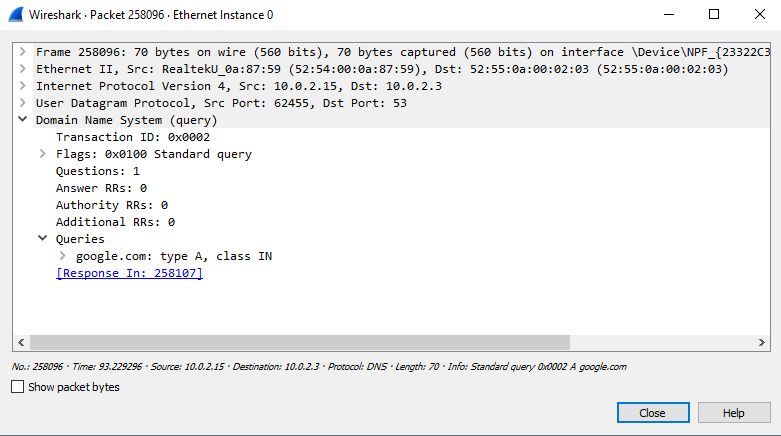
\includegraphics[width=\textwidth]{11}
	 	\caption{Пакет DNS запиту на адресу google.com}
 	\end{minipage}
 	\hfill
	 \begin{minipage}[t]{0.49\textwidth}
	 	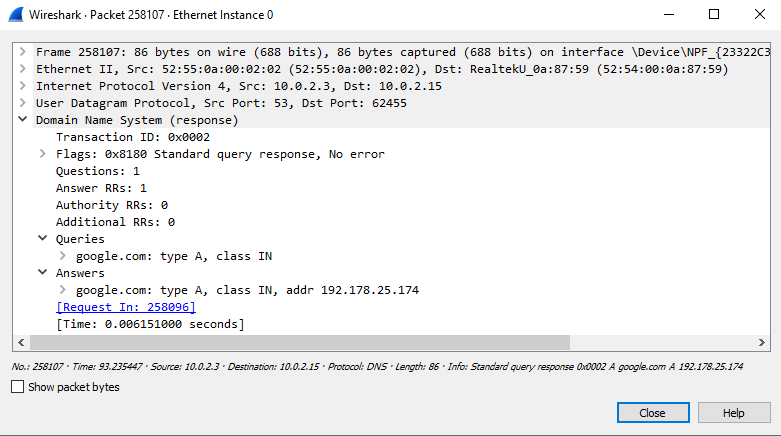
\includegraphics[width=\textwidth]{12}
		\caption{Пакет відповіді на DNS запит від google.com}
	 \end{minipage}
 \end{figure}
 
\begin{figure}[H]
	\centering
	\begin{minipage}[t]{0.49\textwidth}
		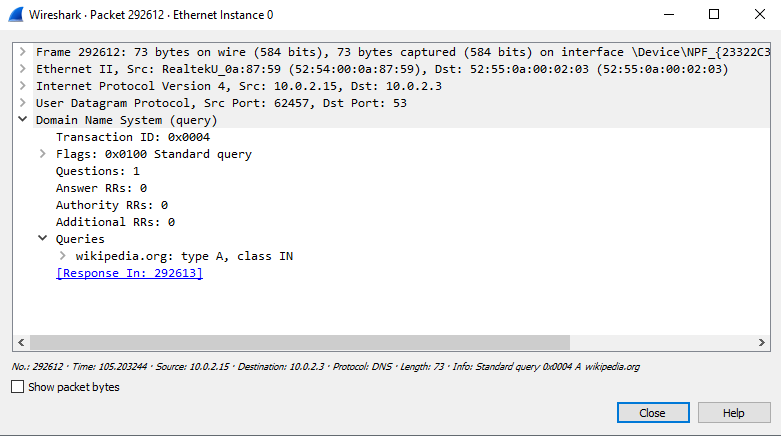
\includegraphics[width=\textwidth]{21}
		\caption{Пакет DNS запиту на адресу wikipedia.org}
	\end{minipage}
	\hfill
	\begin{minipage}[t]{0.49\textwidth}
		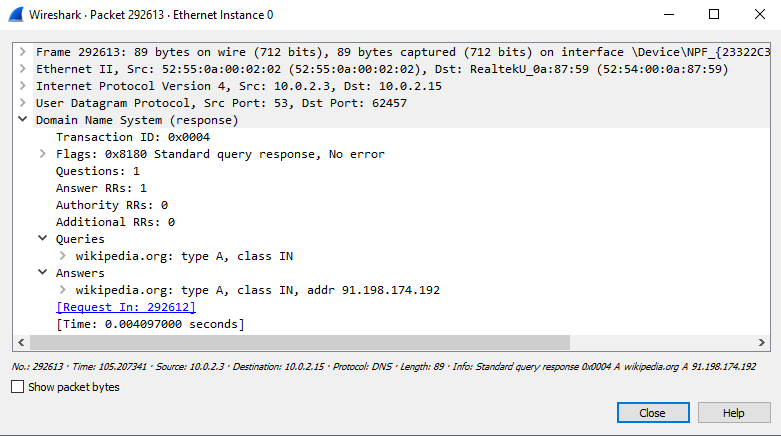
\includegraphics[width=\textwidth]{22}
		\caption{Пакет відповіді на DNS запит від wikipedia.org}
	\end{minipage}
\end{figure}

\begin{figure}[H]
	\centering
	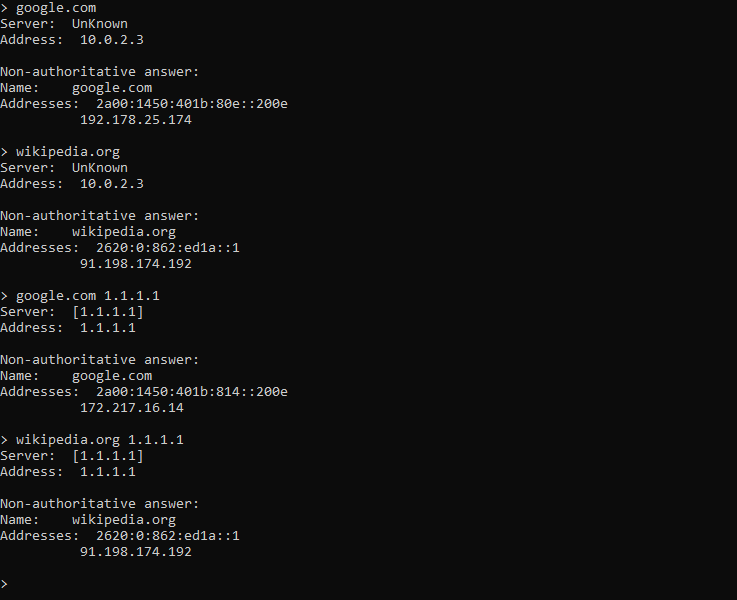
\includegraphics[width=\textwidth]{31}
	\caption{Запитав у DNS-сервера, заданого за замовчуванням, інформацію про доменні імена google.com і wikipedia.org. Запитав цю ж інформацію в іншого DNS-серверів.}
\end{figure}

\begin{figure}[H]
	\centering
	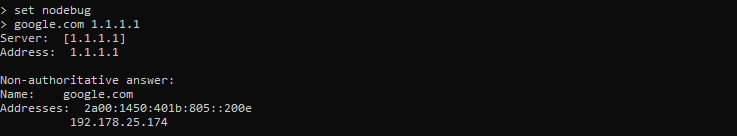
\includegraphics[width=\textwidth]{32}
	\caption{Запит DNS серверу з вимкненим режимом відлагодження}
\end{figure}

\begin{figure}[H]
	\centering
	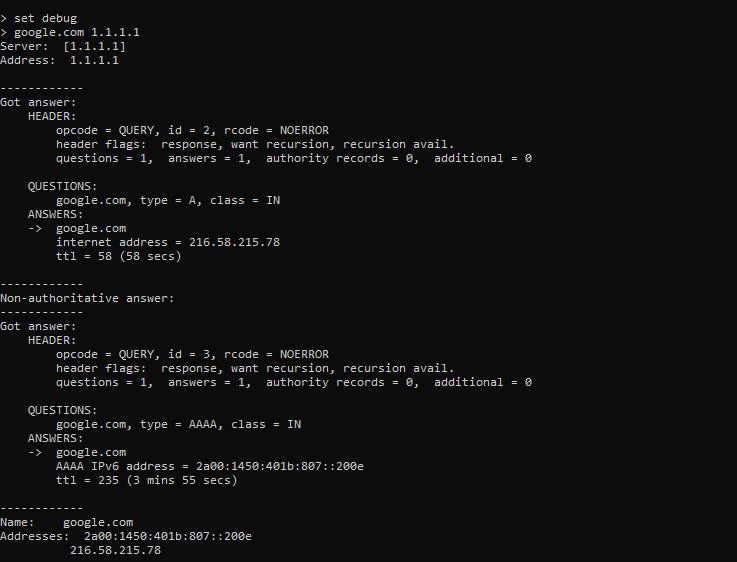
\includegraphics[width=\textwidth]{33}
	\caption{Запит DNS серверу з увімкненим режимом відлагодження}
\end{figure}

\begin{figure}[H]
	\centering
	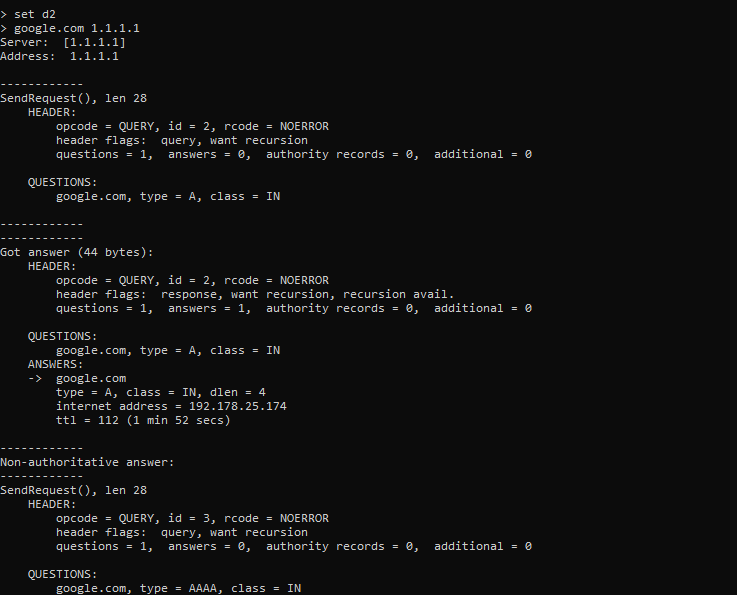
\includegraphics[width=\textwidth]{34}
	\caption{Запит DNS серверу з увімкненим розширеним режимом відлагодження 1/2}
\end{figure}

\begin{figure}[H]
	\centering
	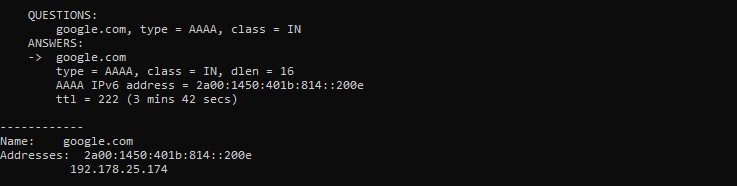
\includegraphics[width=\textwidth]{35}
	\caption{Запит DNS серверу з увімкненим розширеним режимом відлагодження 2/2}
\end{figure}
\begin{figure}[H]
	\centering
	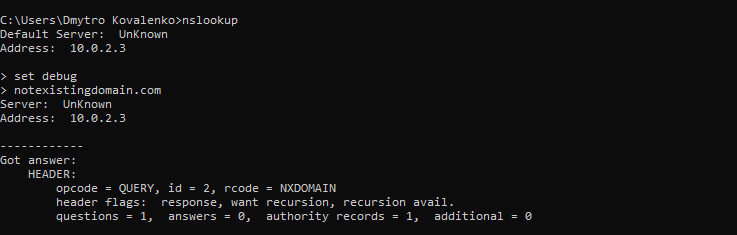
\includegraphics[width=\textwidth]{51}
	\caption{Запит DNS серверу про неіснуючий домен 1/3}
\end{figure}
\begin{figure}[H]
	\centering
	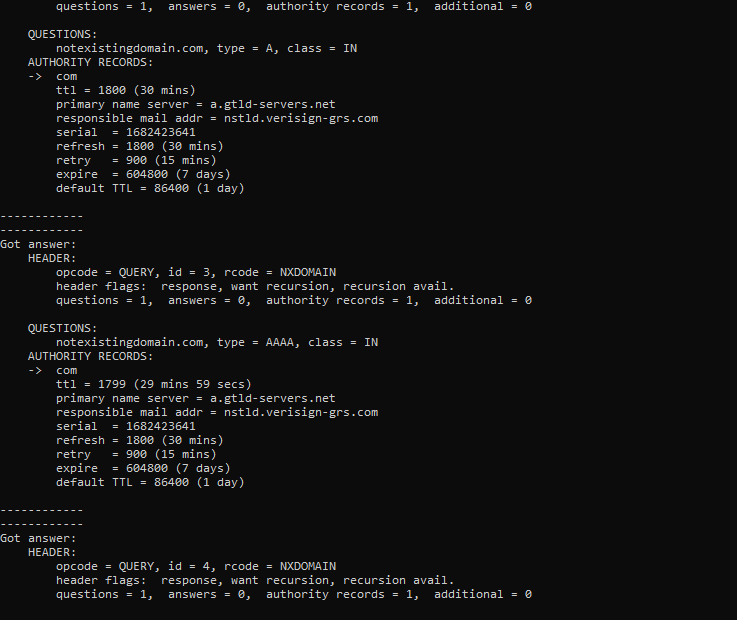
\includegraphics[width=\textwidth]{52}
	\caption{Запит DNS серверу про неіснуючий домен 2/3}
\end{figure}
\begin{figure}[H]
	\centering
	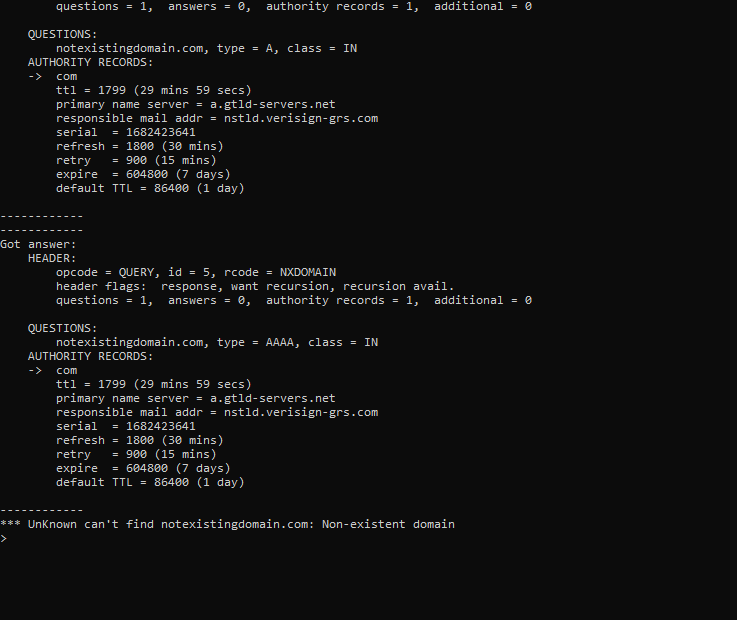
\includegraphics[width=\textwidth]{53}
	\caption{Запит DNS серверу про неіснуючий домен 3/3}
\end{figure}
\begin{figure}[H]
	\centering
	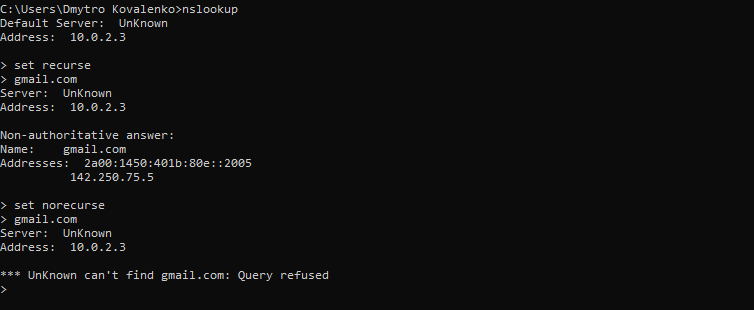
\includegraphics[width=\textwidth]{62}
	\caption{Виконання рекурсивного та нерекурсивного запиту до DNS сервера}
\end{figure}
\begin{figure}[H]
	\centering
	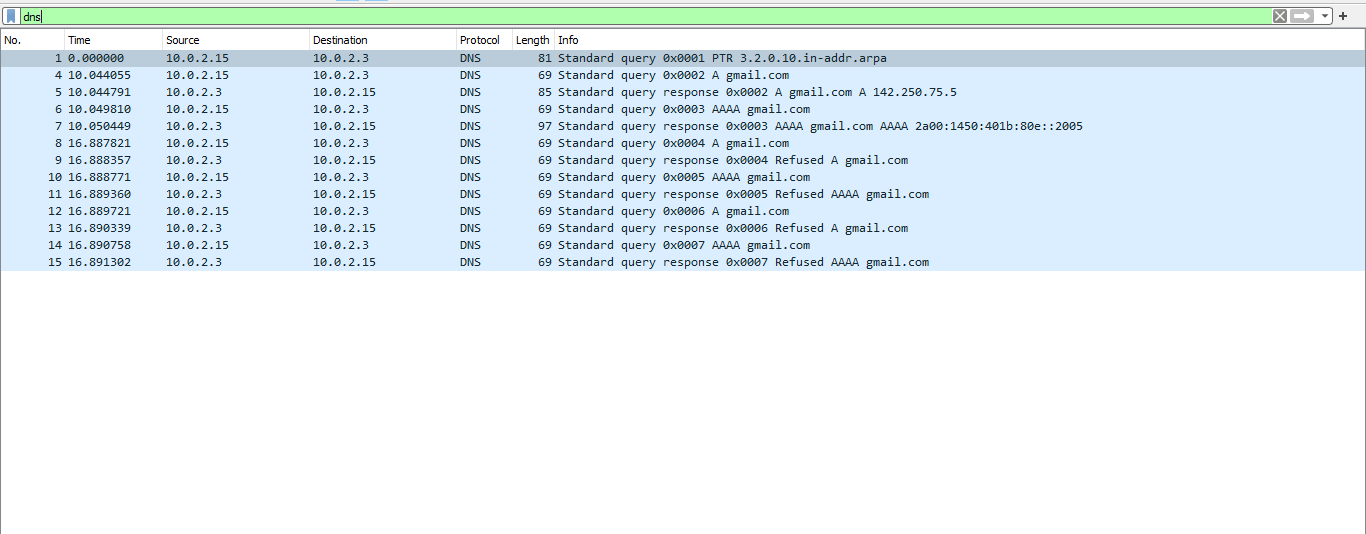
\includegraphics[width=\textwidth]{61}
	\caption{Перехоплені пакети під час виконання рекурсивного та нерекурсивного запиту до DNS сервера}
\end{figure}
\begin{figure}[H]
	\centering
	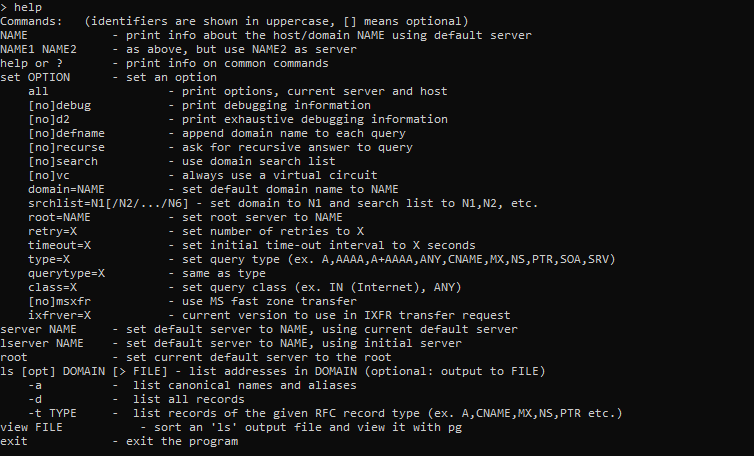
\includegraphics[width=\textwidth]{7}
	\caption{Ознайомився із інформацією про решту ключових слів, що застосовуються з командою set}
\end{figure}
\begin{figure}[H]
	\centering
	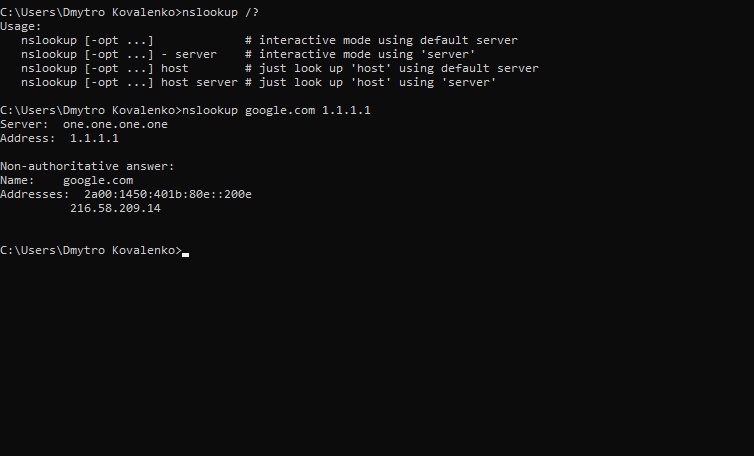
\includegraphics[width=\textwidth]{8}
	\caption{Виконав команди в автономному режимі роботи утиліти nslookup}
\end{figure}

Поясніть передумови виникнення служби DNS і причини, чому схема
розпізнавання IP-адрес за символьними іменами в мережі ARPAnet стала
непрацездатною з ростом числа вузлів.
 
Потрібно було спростити масштабування, адже раніше існував файл hosts.txt, в якому містилася вся інформація про відповідність всіх символьних імен вузлів і їхніх IP-адрес. Цей файл зберігався на одному вузлі мережі ARPAnet і в нього при потребі вносилися зміни. Система ARPAnet вимагала повної таблиці імен на кожному комп'ютера, що було не ефективним з точки зору масштабування.


\section*{Висновки}
Під час виконання лабораторної роботи я вивчив принципи роботи DNS, на практиці ознайомився з принципами роботи DNS-клієнта на прикладі утиліти nslookup, детально дослідив формат DNS-запиту (і відповіді) за допомогою Wireshark і nslookup, а також ознайомився з DHCP повідомленнями.
	    
\end{normalsize}
\end{document}
